\documentclass[11pt]{article}
\usepackage[margin=0.9in]{geometry}
\usepackage{amsmath}
\usepackage{graphicx}
\usepackage{natbib}
\usepackage{hyperref}

\title{LLM Socialnetwork Diffusion\\ Technical Report}
\author{Vince Trencsenyi}
\date{18 August 2026}

\begin{document}

\maketitle
\vspace{-1.5em}

\noindent\textit{Status report on an LLM-enhanced agent-based diffusion model over
the BCDJ microfinance study \citep{Banerjee2013}}

\vspace{0.5em}
\section{Data Interpretation}

A trivial feature analysis based on covariance and variance coverage reveals that household covariates are not strong predictors of adoption rate in the traditional learning sense.
However, in case of LLMs, we may still leverage the demographic information as wealth proxies (\texttt{rooms}, \texttt{beds}, per-capita variants, \texttt{electricity}, \texttt{own\_latrine}, \texttt{occupation\_head}), exposure/attitude to financial services (\texttt{has\_shg}, \texttt{has\_savings}), and in-group/out-group relations (\texttt{subcaste} and \texttt{religion}). In this variant, we consider \texttt{leadership} as an implied feature, rather than an explicit public attribute. This is follows from how the ``leaders'' were chosen based on their occupation, from intution that this feature would have a dominant influence. (Something to be properly investigated in a full project...). Finally, \texttt{adopted} becomes a conditional attribute in the transmission phase. Everything else is dropped: redundant or superseded fields, fields missing in high ratio of records, fields redacted at source, near-constant fields, and bare or vague identifiers.


This study considers the above feature sets not as predictors of adoption, but as foundational traits for grounding the narrative capacity and heterogeneity of the LLMs in plausible, realistic context.

\paragraph{Edge type} In particular, while the type of edge seem like potential predictors and narrative features, we choose not to use them in this variant. Nothing in the survey records who told whom, and the survey didn't ask for justifications. There is no ground truth for which of the twelve relationship types actually carried information or influence. Similarly to the original paper's implementation, here \texttt{informed} is a state, rather than a feature for inference. Consequently, the simulation also runs on the union network rather than trying to select or weight by edge type.

\section{Agent-Based Model}

We take a decision-theoretic approach and seperate the mechanics into two simple ``games''.

\textbf{Transmission}: Every \texttt{informed} household $i$, in each turn, for each (not yet adopted) neighbour $j \in N$ plays the transmission game $G^T = \langle A, S, U_i \rangle$, where the action space is $A=\{\text{ACTIVE},\text{PASSIVE}\}$, the states of nature are $S=\{\text{ADOPTED},\text{NOT ADOPTED}\}$, and the subjective utilities $U$ represent a $\frac{\text{risk}}{\text{reward}}$ relation for the given agent\footnote{Here using the network edge types would likely carry influence that stems from the personal relation of the agents.}. This model builds on the assumption that information transmission is not a neutral act, and the consequences of transmission will yield utility similar to a coordination game (something like~\citep{04edc235-2099-36a0-9888-daf1778d57e4}).

\textbf{Adoption}: Whenever a household $i$ gets \texttt{informed}, it plays the adoption game $G^A = \langle A, S, U_i \rangle$ where the action space -- where the question is \textit{Will this household adopt the microfinance services?} -- is $A=\{\text{YES},\text{NO}\}$, the states of nature pertaining to the potential effects on the household's financial circumstances are $S=\{\text{BENEFICIAL},\text{LIMITED},\text{HARMFUL}\}$, and the subjective utilities $U$ represent a $\frac{\text{risk}}{\text{reward}}$ relation for the given agent. Here, we follow the assumption that the humans will have weighted the potential personal consequences of having access to loans, which on a high-level and time agnostically, can be positive, neutral, or negative.

\section{Agent Design}

Agents are households, not individuals: the individual survey covers only median 46.8\% of a village, albeit non-randomly.
We focus on households and household-aligned features.
household-level representation avoids that, and is also what the
time and resources here could support. 


\paragraph{A Note on Implementation}
I prefer to use strongly structured (as per old-school Wooldridge) agent architectures wrapping LLMs, rather than assuming inherent agency off-the shelf.
This use case nicely aligns with the specific Observe--Orient--Decide--Act cycle I like to use where we can model cognitive and physical features, and account for environmental uncertainties.
While the sequential model still follows this concept and the round protocol (receive, decide, advance) is loosely OODA-shaped, this is not implemented here due to the time and complexity overhead.
Design choices here pertain to the use of a hybrid algorithmic+neural (LLM) agents or the purely synthetic autonomous LLM population (\textbf{W.I.P.}), and to a narrow selection of prompt designs covering ideas from information sets, cognitive theory and decision theory.

\section{Experiment Design}

The initial choice is \textbf{Village 6}. This is based on capita and edge count, not on data quality.
At a five-round horizon its 730-edge network needs 3{,}650 edge-round calls against 7{,}824 (village 47)
and 12{,}132 (village 73). The trade-off is the lower survey coverage of households.

\textbf{Timing is not real}: $q_N,q_P$ were fit to reproduce the eventual adoption pattern, not a documented sequence of conversations.
While we adpopt the rounds $=$ trimester presence count assumption from the papers, the household-level adoption record and the panel's trimester curve are two different empirical objects, so simulated trajectory is to beviewed as a modelling artefact (albeit interesting!) rather than objective measure of human-likeness in this study.

\textbf{Adoption rate pilot.} Due to the cost and time constraints, we first conduct a pilot to narrow down agent selection for a more extensive simulation, scored on whether an LLM decision tells apart a real adopter from a real non-adopter, on \texttt{gpt-5.4-nano} at $n=20$ per axess (Figure~\ref{fig:pilot}).

\begin{description}
    \item[Ego profile]:
    \begin{description}
        \item[0]: No household info involved.
        \item[1]: Data incorporated as a listing.
        \item[2]: Data incorporated as and engaging narrative story.   
    \end{description}
    \item[Neighbour profile]: Same as above.
    \item[Endorsement]:
    \begin{description}
        \item[0]: What the neighbour decided is not mentioned.
        \item[1]: The neighbour's decision is mentioned.  
    \end{description}
    \item[Response format]:
    \begin{description}
        \item[0]Plain: Vanilla prompt.
        \item[1]Model of appropriateness: The agent answers 1. What kind of situation is this? 2. What kind of person am I? 3. What should someone like me do in a situation like this?
        \item[2]Decision-theoretic: The LLM must provide a structured JSON schema, populating a decision matrix according to the game definitions, providing a justification for each selected value.   
    \end{description}
\end{description}


Results from the pilot are consistent with an earlier finding in~\citep{Trencsenyi2025}, such that the complexity of the agent model and the human-likeness of the results do not have an obvious monotonic relationship, the evaluation is sensitive to metric and objective. Quite often higher complexity triggers the LLM being overly strategic making it less human-like.

\begin{figure}[h]
  \centering
  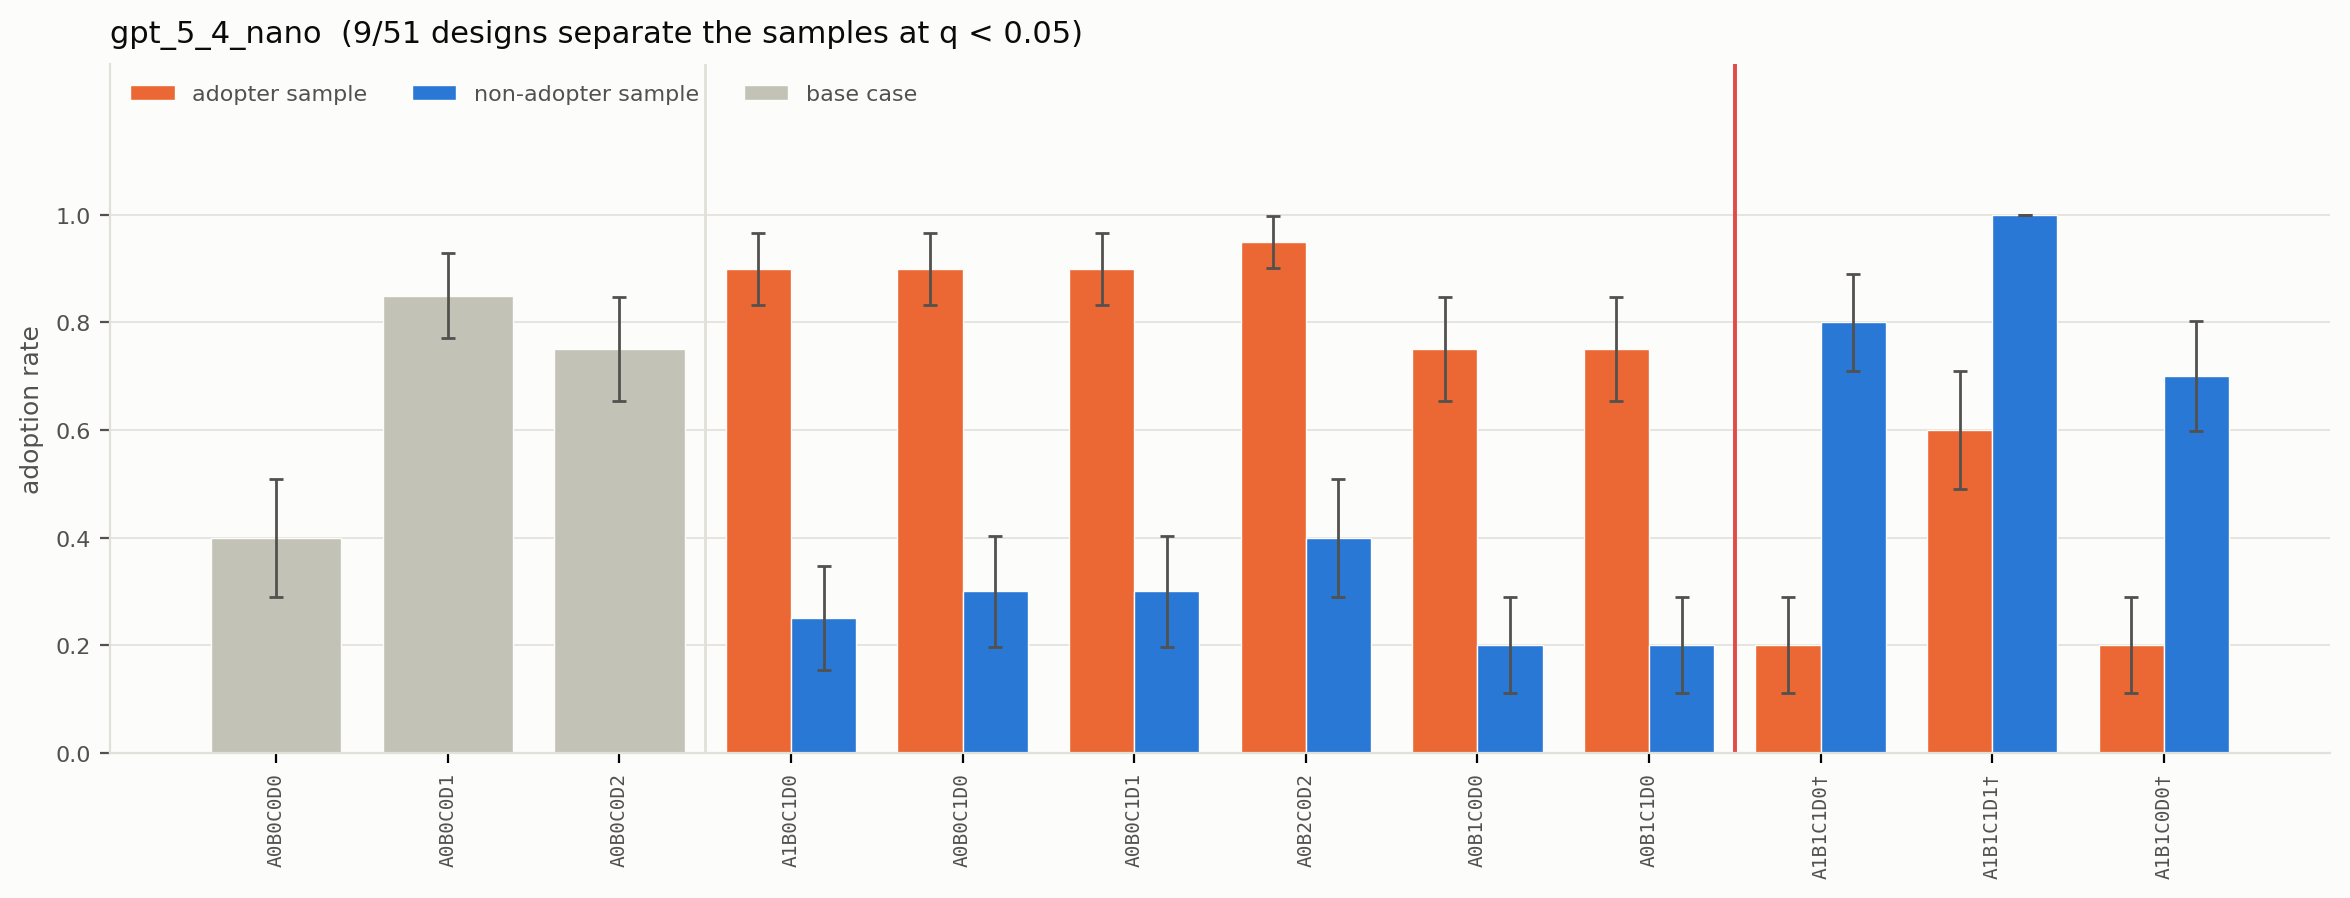
\includegraphics[width=0.92\textwidth]{../figures/pilot/adoption_rates_fisher.png}
  \vspace{-0.3em}
  \caption{Adoption rate by design, filtered by statistical significance, adopter vs.\ non-adopter sample
  household, $n=20$ reps/arm. Grey: base cases. Red line: designs that invert.}
  \label{fig:pilot}
\end{figure}

For a full project, four extensions follow: log-probability shifts from
SHG/bank-account toggles on engineered minimal pairs at temperature zero;
folding the LOA questions into the decision-theoretic matrix;
explicit belief elicitation (skipped by default -- it biased responses
heavily toward one outcome); less-constrained and smaller models (both
found more human-like in my previous studies); and whether leadership must be stated
explicitly or can be inferred from occupation.

\textbf{Hybrid model.} Of two transmission variants, one is built: each
household is prompted once, when first informed, never again ---
BCDJ's \texttt{contagiousbefore} rule exactly. The other, BCDJ's endorsement
model (``how many told me''), is a stub (\texttt{NotImplementedError})
pending a belief-update model; what exists is narrower, a toggle disclosing
one informer's status. The true ``share of informers who joined'' is
recoverable only from logs after a run, never shown to the agent. Runs are
pruned to the giant component (village 6: 107/114), matching BCDJ's
convention. Only \texttt{gpt-5.4-nano} is wired in, and no scorer against
ground truth exists yet --- the run-record schema is built for one.

\textbf{Synthetic population} under construction, subject to results from hybrid.

\section{First glance on potential stretch}

The demographic-plus-network-plus-adoption structure here has cousins in experimental economics with WEIRD-population demographic data, a possible route to a Western comparison population via public goods games, and signalling games, or other canonical multi-stage-game sequential interaction models.

{\small
\bibliographystyle{plainnat}
\bibliography{references}
}

\end{document}
